% ========== RÅBUK ==========
\begin{frame}{%
  \begin{minipage}[c]{0.30\textwidth}
    Råbuk
  \end{minipage}%
  \hfill
  \begin{minipage}[c]{0.45\textwidth}
    \footnotesize
    \textbf{Jagttid:} 16.\ maj -- 15.\ jul.\\
    samt 1.\ okt.--31.\ jan.
  \end{minipage}%
  \hfill
  \begin{minipage}[c]{0.15\textwidth}
    \noindent\raggedleft
    
\includegraphics[width=0.5cm, height=0.5cm, keepaspectratio]{Billeder/Ikoner/star.png}%
    \hspace{0.2em}%
    
\includegraphics[width=0.5cm, height=0.5cm, keepaspectratio]{Billeder/Ikoner/star.png}%
    \hspace{0.2em}%
    
\includegraphics[width=0.5cm, height=0.5cm, keepaspectratio]{Billeder/Ikoner/star.png}
  \end{minipage}%
}
  \vspace{0.25em}
  \begin{columns}[T]
    \column{0.45\textwidth}
    \setlength{\parskip}{0.4em}
    \tiny
    \RaggedRight
    \textbf{\textit{Capreolus capreolus}} – mindste hjorteart i Danmark. Hannen kaldes råbuk og kendes på det lille gevir. I andet leveår kaldes den spidsbuk. \par
    \textbf{Udseende:}\\
    \quad – Kort snudeskaft med sort plet \\
    \quad – Gulligt/hvidt spejl \\
    \quad – Rødbrun/grå \par
    \textbf{Levesteder:} Randzoner og nye skovarealer. Mest aktiv morgen og aften. \par
    \textbf{Føde:} Græsser, urter, knopper og skud fra buske. \par
    \textbf{Udbredelse:} Hele landet. \par
    \textbf{Yngleforhold:} Forlænget drægtighed. \par
    \textbf{Parring/brunst:} Slutningen af juli / starten af august. \par
    \textbf{Sygdomme:} Svælgbremser, pelslus
    \textbf{Forplantning:}\\
    \quad – \textbf{Kønsmoden:} 1 år \\
    \quad – \textbf{Mono/polygam:} Polygam \\
    \quad – \textbf{Bestandsomsætning:} Hurtig \\
    \quad – \textbf{Kuld:} 1--3 lam, oftest 2 \par
    %\textbf{*Bemærk:} Lokale jagttider kan forekomme.
    \column{0.52\textwidth}
    \centering
    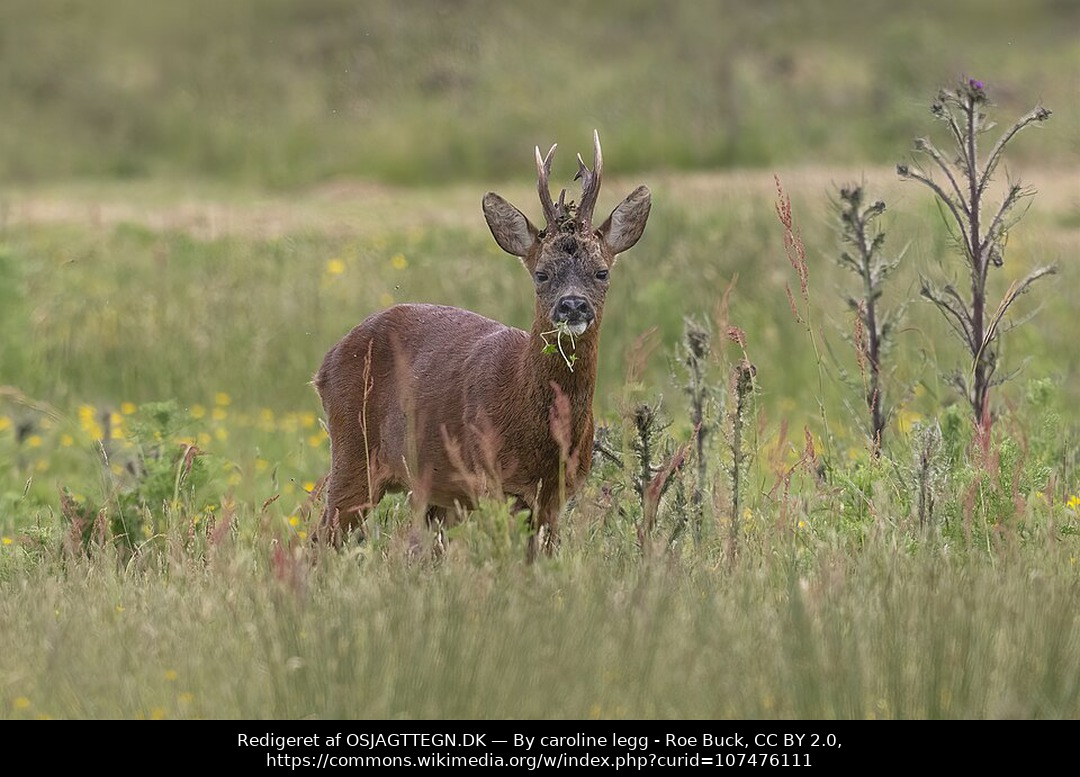
\includegraphics[width=\linewidth, height=7.2cm, keepaspectratio]{Billeder/Dyr/Pattedyr/hovdyr/råvildt/raavildt-male-10.jpg}
  \end{columns}
\end{frame}